% Options for packages loaded elsewhere
% Options for packages loaded elsewhere
\PassOptionsToPackage{unicode}{hyperref}
\PassOptionsToPackage{hyphens}{url}
\PassOptionsToPackage{dvipsnames,svgnames,x11names}{xcolor}
%
\documentclass[
  11pt,
  letterpaper,
  DIV=11,
  numbers=noendperiod]{scrartcl}
\usepackage{xcolor}
\usepackage[margin=1in]{geometry}
\usepackage{amsmath,amssymb}
\setcounter{secnumdepth}{-\maxdimen} % remove section numbering
\usepackage{iftex}
\ifPDFTeX
  \usepackage[T1]{fontenc}
  \usepackage[utf8]{inputenc}
  \usepackage{textcomp} % provide euro and other symbols
\else % if luatex or xetex
  \usepackage{unicode-math} % this also loads fontspec
  \defaultfontfeatures{Scale=MatchLowercase}
  \defaultfontfeatures[\rmfamily]{Ligatures=TeX,Scale=1}
\fi
\usepackage{lmodern}
\ifPDFTeX\else
  % xetex/luatex font selection
  \setmainfont[]{TeX Gyre Heros}
  \setsansfont[]{TeX Gyre Heros}
\fi
% Use upquote if available, for straight quotes in verbatim environments
\IfFileExists{upquote.sty}{\usepackage{upquote}}{}
\IfFileExists{microtype.sty}{% use microtype if available
  \usepackage[]{microtype}
  \UseMicrotypeSet[protrusion]{basicmath} % disable protrusion for tt fonts
}{}
\makeatletter
\@ifundefined{KOMAClassName}{% if non-KOMA class
  \IfFileExists{parskip.sty}{%
    \usepackage{parskip}
  }{% else
    \setlength{\parindent}{0pt}
    \setlength{\parskip}{6pt plus 2pt minus 1pt}}
}{% if KOMA class
  \KOMAoptions{parskip=half}}
\makeatother
% Make \paragraph and \subparagraph free-standing
\makeatletter
\ifx\paragraph\undefined\else
  \let\oldparagraph\paragraph
  \renewcommand{\paragraph}{
    \@ifstar
      \xxxParagraphStar
      \xxxParagraphNoStar
  }
  \newcommand{\xxxParagraphStar}[1]{\oldparagraph*{#1}\mbox{}}
  \newcommand{\xxxParagraphNoStar}[1]{\oldparagraph{#1}\mbox{}}
\fi
\ifx\subparagraph\undefined\else
  \let\oldsubparagraph\subparagraph
  \renewcommand{\subparagraph}{
    \@ifstar
      \xxxSubParagraphStar
      \xxxSubParagraphNoStar
  }
  \newcommand{\xxxSubParagraphStar}[1]{\oldsubparagraph*{#1}\mbox{}}
  \newcommand{\xxxSubParagraphNoStar}[1]{\oldsubparagraph{#1}\mbox{}}
\fi
\makeatother

\usepackage{color}
\usepackage{fancyvrb}
\newcommand{\VerbBar}{|}
\newcommand{\VERB}{\Verb[commandchars=\\\{\}]}
\DefineVerbatimEnvironment{Highlighting}{Verbatim}{commandchars=\\\{\}}
% Add ',fontsize=\small' for more characters per line
\usepackage{framed}
\definecolor{shadecolor}{RGB}{241,243,245}
\newenvironment{Shaded}{\begin{snugshade}}{\end{snugshade}}
\newcommand{\AlertTok}[1]{\textcolor[rgb]{0.68,0.00,0.00}{#1}}
\newcommand{\AnnotationTok}[1]{\textcolor[rgb]{0.37,0.37,0.37}{#1}}
\newcommand{\AttributeTok}[1]{\textcolor[rgb]{0.40,0.45,0.13}{#1}}
\newcommand{\BaseNTok}[1]{\textcolor[rgb]{0.68,0.00,0.00}{#1}}
\newcommand{\BuiltInTok}[1]{\textcolor[rgb]{0.00,0.23,0.31}{#1}}
\newcommand{\CharTok}[1]{\textcolor[rgb]{0.13,0.47,0.30}{#1}}
\newcommand{\CommentTok}[1]{\textcolor[rgb]{0.37,0.37,0.37}{#1}}
\newcommand{\CommentVarTok}[1]{\textcolor[rgb]{0.37,0.37,0.37}{\textit{#1}}}
\newcommand{\ConstantTok}[1]{\textcolor[rgb]{0.56,0.35,0.01}{#1}}
\newcommand{\ControlFlowTok}[1]{\textcolor[rgb]{0.00,0.23,0.31}{\textbf{#1}}}
\newcommand{\DataTypeTok}[1]{\textcolor[rgb]{0.68,0.00,0.00}{#1}}
\newcommand{\DecValTok}[1]{\textcolor[rgb]{0.68,0.00,0.00}{#1}}
\newcommand{\DocumentationTok}[1]{\textcolor[rgb]{0.37,0.37,0.37}{\textit{#1}}}
\newcommand{\ErrorTok}[1]{\textcolor[rgb]{0.68,0.00,0.00}{#1}}
\newcommand{\ExtensionTok}[1]{\textcolor[rgb]{0.00,0.23,0.31}{#1}}
\newcommand{\FloatTok}[1]{\textcolor[rgb]{0.68,0.00,0.00}{#1}}
\newcommand{\FunctionTok}[1]{\textcolor[rgb]{0.28,0.35,0.67}{#1}}
\newcommand{\ImportTok}[1]{\textcolor[rgb]{0.00,0.46,0.62}{#1}}
\newcommand{\InformationTok}[1]{\textcolor[rgb]{0.37,0.37,0.37}{#1}}
\newcommand{\KeywordTok}[1]{\textcolor[rgb]{0.00,0.23,0.31}{\textbf{#1}}}
\newcommand{\NormalTok}[1]{\textcolor[rgb]{0.00,0.23,0.31}{#1}}
\newcommand{\OperatorTok}[1]{\textcolor[rgb]{0.37,0.37,0.37}{#1}}
\newcommand{\OtherTok}[1]{\textcolor[rgb]{0.00,0.23,0.31}{#1}}
\newcommand{\PreprocessorTok}[1]{\textcolor[rgb]{0.68,0.00,0.00}{#1}}
\newcommand{\RegionMarkerTok}[1]{\textcolor[rgb]{0.00,0.23,0.31}{#1}}
\newcommand{\SpecialCharTok}[1]{\textcolor[rgb]{0.37,0.37,0.37}{#1}}
\newcommand{\SpecialStringTok}[1]{\textcolor[rgb]{0.13,0.47,0.30}{#1}}
\newcommand{\StringTok}[1]{\textcolor[rgb]{0.13,0.47,0.30}{#1}}
\newcommand{\VariableTok}[1]{\textcolor[rgb]{0.07,0.07,0.07}{#1}}
\newcommand{\VerbatimStringTok}[1]{\textcolor[rgb]{0.13,0.47,0.30}{#1}}
\newcommand{\WarningTok}[1]{\textcolor[rgb]{0.37,0.37,0.37}{\textit{#1}}}

\usepackage{longtable,booktabs,array}
\newcounter{none} % for unnumbered tables
\usepackage{calc} % for calculating minipage widths
% Correct order of tables after \paragraph or \subparagraph
\usepackage{etoolbox}
\makeatletter
\patchcmd\longtable{\par}{\if@noskipsec\mbox{}\fi\par}{}{}
\makeatother
% Allow footnotes in longtable head/foot
\IfFileExists{footnotehyper.sty}{\usepackage{footnotehyper}}{\usepackage{footnote}}
\makesavenoteenv{longtable}
\usepackage{graphicx}
\makeatletter
\newsavebox\pandoc@box
\newcommand*\pandocbounded[1]{% scales image to fit in text height/width
  \sbox\pandoc@box{#1}%
  \Gscale@div\@tempa{\textheight}{\dimexpr\ht\pandoc@box+\dp\pandoc@box\relax}%
  \Gscale@div\@tempb{\linewidth}{\wd\pandoc@box}%
  \ifdim\@tempb\p@<\@tempa\p@\let\@tempa\@tempb\fi% select the smaller of both
  \ifdim\@tempa\p@<\p@\scalebox{\@tempa}{\usebox\pandoc@box}%
  \else\usebox{\pandoc@box}%
  \fi%
}
% Set default figure placement to htbp
\def\fps@figure{htbp}
\makeatother


% definitions for citeproc citations
\NewDocumentCommand\citeproctext{}{}
\NewDocumentCommand\citeproc{mm}{%
  \begingroup\def\citeproctext{#2}\cite{#1}\endgroup}
\makeatletter
 % allow citations to break across lines
 \let\@cite@ofmt\@firstofone
 % avoid brackets around text for \cite:
 \def\@biblabel#1{}
 \def\@cite#1#2{{#1\if@tempswa , #2\fi}}
\makeatother
\newlength{\cslhangindent}
\setlength{\cslhangindent}{1.5em}
\newlength{\csllabelwidth}
\setlength{\csllabelwidth}{3em}
\newenvironment{CSLReferences}[2] % #1 hanging-indent, #2 entry-spacing
 {\begin{list}{}{%
  \setlength{\itemindent}{0pt}
  \setlength{\leftmargin}{0pt}
  \setlength{\parsep}{0pt}
  % turn on hanging indent if param 1 is 1
  \ifodd #1
   \setlength{\leftmargin}{\cslhangindent}
   \setlength{\itemindent}{-1\cslhangindent}
  \fi
  % set entry spacing
  \setlength{\itemsep}{#2\baselineskip}}}
 {\end{list}}
\usepackage{calc}
\newcommand{\CSLBlock}[1]{\hfill\break\parbox[t]{\linewidth}{\strut\ignorespaces#1\strut}}
\newcommand{\CSLLeftMargin}[1]{\parbox[t]{\csllabelwidth}{\strut#1\strut}}
\newcommand{\CSLRightInline}[1]{\parbox[t]{\linewidth - \csllabelwidth}{\strut#1\strut}}
\newcommand{\CSLIndent}[1]{\hspace{\cslhangindent}#1}



\setlength{\emergencystretch}{3em} % prevent overfull lines

\providecommand{\tightlist}{%
  \setlength{\itemsep}{0pt}\setlength{\parskip}{0pt}}



 


\KOMAoption{captions}{tableheading}
\makeatletter
\@ifpackageloaded{tcolorbox}{}{\usepackage[skins,breakable]{tcolorbox}}
\@ifpackageloaded{fontawesome5}{}{\usepackage{fontawesome5}}
\definecolor{quarto-callout-color}{HTML}{909090}
\definecolor{quarto-callout-note-color}{HTML}{0758E5}
\definecolor{quarto-callout-important-color}{HTML}{CC1914}
\definecolor{quarto-callout-warning-color}{HTML}{EB9113}
\definecolor{quarto-callout-tip-color}{HTML}{00A047}
\definecolor{quarto-callout-caution-color}{HTML}{FC5300}
\definecolor{quarto-callout-color-frame}{HTML}{acacac}
\definecolor{quarto-callout-note-color-frame}{HTML}{4582ec}
\definecolor{quarto-callout-important-color-frame}{HTML}{d9534f}
\definecolor{quarto-callout-warning-color-frame}{HTML}{f0ad4e}
\definecolor{quarto-callout-tip-color-frame}{HTML}{02b875}
\definecolor{quarto-callout-caution-color-frame}{HTML}{fd7e14}
\makeatother
\makeatletter
\@ifpackageloaded{caption}{}{\usepackage{caption}}
\AtBeginDocument{%
\ifdefined\contentsname
  \renewcommand*\contentsname{Table of contents}
\else
  \newcommand\contentsname{Table of contents}
\fi
\ifdefined\listfigurename
  \renewcommand*\listfigurename{List of Figures}
\else
  \newcommand\listfigurename{List of Figures}
\fi
\ifdefined\listtablename
  \renewcommand*\listtablename{List of Tables}
\else
  \newcommand\listtablename{List of Tables}
\fi
\ifdefined\figurename
  \renewcommand*\figurename{Figure}
\else
  \newcommand\figurename{Figure}
\fi
\ifdefined\tablename
  \renewcommand*\tablename{Table}
\else
  \newcommand\tablename{Table}
\fi
}
\@ifpackageloaded{float}{}{\usepackage{float}}
\floatstyle{ruled}
\@ifundefined{c@chapter}{\newfloat{codelisting}{h}{lop}}{\newfloat{codelisting}{h}{lop}[chapter]}
\floatname{codelisting}{Listing}
\newcommand*\listoflistings{\listof{codelisting}{List of Listings}}
\makeatother
\makeatletter
\makeatother
\makeatletter
\@ifpackageloaded{caption}{}{\usepackage{caption}}
\@ifpackageloaded{subcaption}{}{\usepackage{subcaption}}
\makeatother
\usepackage{bookmark}
\IfFileExists{xurl.sty}{\usepackage{xurl}}{} % add URL line breaks if available
\urlstyle{same}
\hypersetup{
  pdftitle={L15 · Energy minimization with many coordinates},
  colorlinks=true,
  linkcolor={blue},
  filecolor={Maroon},
  citecolor={Blue},
  urlcolor={Blue},
  pdfcreator={LaTeX via pandoc}}


\title{L15 · Energy minimization with many coordinates}
\usepackage{etoolbox}
\makeatletter
\providecommand{\subtitle}[1]{% add subtitle to \maketitle
  \apptocmd{\@title}{\par {\large #1 \par}}{}{}
}
\makeatother
\subtitle{From force balance to the Hessian and numerical optimization}
\author{}
\date{}
\begin{document}
\maketitle


\begin{tcolorbox}[enhanced jigsaw, arc=.35mm, bottomrule=.15mm, bottomtitle=1mm, breakable, colback=white, colbacktitle=quarto-callout-note-color!10!white, colframe=quarto-callout-note-color-frame, coltitle=black, left=2mm, leftrule=.75mm, opacityback=0, opacitybacktitle=0.6, rightrule=.15mm, title=\textcolor{quarto-callout-note-color}{\faInfo}\hspace{0.5em}{Central question}, titlerule=0mm, toprule=.15mm, toptitle=1mm]

\textbf{Given the energy of an atomic system, how can we calculate a
stable structure, and where do matrix solves enter the optimization?}

\end{tcolorbox}

\subsection{Learning outcomes}\label{learning-outcomes}

By the end of this lecture, you should be able to:

\begin{enumerate}
\def\labelenumi{\arabic{enumi}.}
\tightlist
\item
  \textbf{Derive} the Newton equation
  \(\mathbf H\Delta\mathbf x=-\nabla E\) from force balance and identify
  the Hessian.
\item
  \textbf{Compare} the constant Hessian of a quadratic energy with the
  changing Hessian of a geometrically nonlinear spring system.
\item
  \textbf{Minimize} a supplied two-coordinate energy with SciPy,
  choosing the energy and derivative inputs appropriate to the method.
\item
  \textbf{Distinguish} a local minimum from a saddle point using the
  energy changes around a converged structure.
\end{enumerate}

\subsection{From force balance to energy
minimization}\label{from-force-balance-to-energy-minimization}

In L14, we demonstrated how to solve a non-linear system of equations by
demonstrating chain of atoms under external force. We're solving a sets
of equations

F\_i (\matbbf) = F\_int\_i(\mathbf) - f\_i = 0

And we showed that using newton's method on high-dimesions, it is
possible to convert to a linear matrix solving problem wen updating each
step from a guess

xm+1 = x\_m + Delta x J Delta x = -F(x)

Newton's method did this by repeatedly solving a linear system involving
the Jacobian of the force. We wanted to note \(J\) is the jacobian of
the net force, and it needs to be updated everytime.

One direct extension to this is when external force f = 0, what do we
solve is now essentially the local minimum structure. Since we showed

F\_int\_i = -\partial E/\partial x\_i

solving F\_i = F\_int\_i = 0 is basically related to solve

partial E/partial x\_i = 0 \ldots{}

This is a \textbf{relaxation problem}, which is the core to any
materials simulations. Relaxing the force of a system, is equivalent to
find the \textbf{minimization} of the total energy of an atomistic
system.

\textless box this --\textgreater{}

Relaxation in force \textless--\textgreater{} minimize energy (second
row) Solve \partia E/\partialx  minE

\textless call-out tip Newtonian vs Hamiltonian views (just anecdote)

Historically there are newtonian and hamiltonian ways od describing a
many body system; in laymen's words - newtonian (force analysis):
knowing all the forces in the many bodies - hamiltonian (): \ldots{}
\textgreater{}

\subsubsection{Recapping local vs global
minima}\label{recapping-local-vs-global-minima}

We have briefly seen this concept in both lecture 07 and assignment 1.
In a many atom / high-dimensional coordination system, solving force = 0
does not necessariely ean we could find the structure with energy lowest
from all possible geometries.

\begin{itemize}
\tightlist
\item
  Local minimum: this is a position x\_m, that moving any infinitely
  small displacement Delta x from it, will cause energy to increase.
  \emph{howver}, local mimimum does not guarenteem there wil be pos,
  that a large enough displacement x\_m + Delta x will have lower energy
\item
  Global minimum: lowest energy among all allowed configurations
  (e.g.~search all possible values (x1, x2, \ldots{} xN))
\end{itemize}

For higher dimension structures, it is very likely an initial pos only
get to a local minimum. changing a different start point will likely go
down to a better minimum, but to trly find the global minimum, is a hard
task and beyond this course's context. For interested, please see
methods like .

\subsubsection{Ensuring minimum: second
derivative}\label{ensuring-minimum-second-derivative}

From the minimization in 1D, we know that the having f'(x) = 0 is not
enough, we have to have f'\,'(x) \textgreater{} 0 to ensure it's indeed
a minimum.

The same thing occurs for minimization in higher dimension as well. We
want the second derivative of energy to be positive in \textbf{all
directions} to make sure it's minimum. This is a slightly different
focus of problem, so we will discuss it in L16 using the concept of
eigenvalue analysis.

\subsection{Minimization of energy: the Newton-Raphson
Approach}\label{minimization-of-energy-the-newton-raphson-approach}

For this class, let's consider a slightly more interesting question: 3
atoms in a line, with the end atoms fixed, the middle atom able to move
freely in either x- or y- directions. The total energy between the aomts
E(x, y) has a generally non-linear form, that we will not reveal first.

\subsubsection{2D system basic concepts}\label{d-system-basic-concepts}

There are some concepts in the vector calculus that may find useful.
Using the 2D coordinate (x, y)

\textbf{Gradient}, is basically a vector \nabla E =
{[}\partial E/partial x, \partial E/\partial y{]}

In the case of 2 free coordinates, the internal force F(x, y) just F(x,
y) = -nabla E = {[}-partal / partial x, -partial / partial y{]}

The gradient tells us how large the internal force, and geometrically
the local slope of the energy ``surface''

\textbf{Hessian matrix}, which is matrix of second derivative with
respect to the energy.

H = {[}partial\^{}2 E/partial x\^{}2, \ldots;\ldots;;\ldots{]}

the hessian matrix tells us about the curvature of the energy surface.
Numerically, it is just the negative of the Jacboan matrix of force

H = -J\_F = \ldots{}

we used the notation J\_F to say its jacobian of the force, just to be
distinct.

There are many ways to intuitively understand the hessian, for example
1. it means how fast the energy will increase in different directions
(larger magnitude of hessian --\textgreater{} quicker ) 2. it means the
local curvature (how bended) the energy surface is (larger magnitude of
hessian --\textgreater{} more bended) 3. for atomic systems it is
related to the local spring constant (larger magnitude of
hessian--\textgreater{} stiffer)

\textless callout fold why?

the energy near \textbf{the minimum} can be approximated using the
taylor's expansion method

E(Delta x, Delta y) = E\_min + 1/2Delta x\^{}THDelta x

a higher magnitude \textless in fact what? norm? determinant?
eigenvalue?\textgreater{} will mean the energy increase steep

\begin{quote}
\end{quote}

\subsubsection{Minimization in newton's
method}\label{minimization-in-newtons-method}

Recall that in newton's method, we need to solve

J\_F \Delta x = -F(x)

in energy's term, we just write

H \Delta x = \nabla E(x)

and that is all what we need to minimize. in 2D, basically

{[}2D matrix of hessian{]} Delta x = {[}2 row nabla E{]}

why bother rewrite the equation again? We can show that it is basically
just knowing

E(x, y) as a scalar, and then we can minimize everything from this
multi-dimensional energy function

\textless call out: relation to 1D newton method

in lecture 7 we said newton's method builds on both 1d and 2d derivative
f' and f'\,'

x\_m+1 = x\_m - f'/f'\,'

analogously in multidim

x = xm - H\^{}-1 E

although in fact we do not solve the inverse of hessian \textgreater{}

\subsection{Miniminzation in Numpy
library}\label{miniminzation-in-numpy-library}

Newton's method is cool, and we can indeed use scipy.optimize.newton to
do it.

In many cases the gradient and hessian might be difficult to write
explicitly, scipy provides many other functions to do this

scipy.optimize.minimize will be very good at it

You have already use it for minimizing the fitting coefficients in
assignemtn 2. to optimize the atomic sturctures, similar can also be
used

\subsection{Demo: One moving atom with two
coordinates}\label{demo-one-moving-atom-with-two-coordinates}

Let's reveal out toy system! \textless for this system let's don't say
which kind of energy E form we would have, even though could use
spring\textgreater{}

\textless fix this demo, so that student can artificial make atoms
apart, and see how newton try to find the minima\textgreater{}

\textless the supplied atomic system will use a dropdown to reveal what
energy form used, including spring const, LJ, and a cheap
morse\textgreater{}

\textless we don't show how to minimize a real atom systems yet! no bfgs
etcetc\textgreater{}

\textless for each system, we will provide the function for gradient and
hessian\textgreater{}

Ask students to predict where the minimum will be, by changing the
parameter a (whether initially compressed or stretched, they shall see
the diff)

\begin{figure}

\centering{

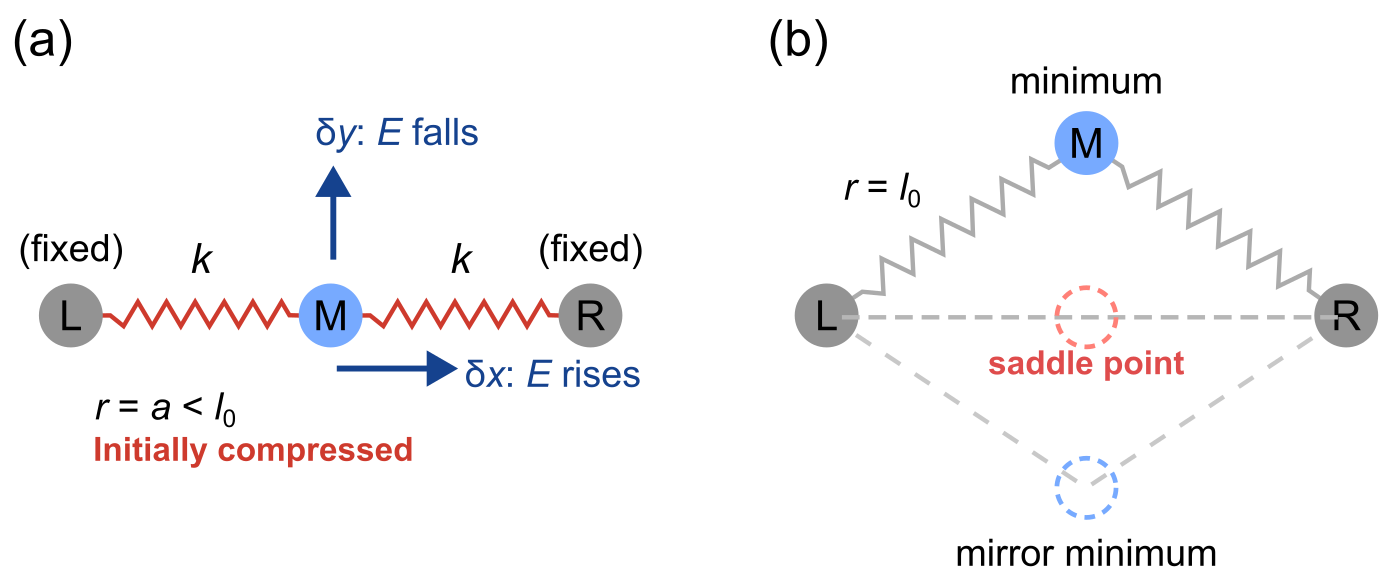
\includegraphics[width=0.9\linewidth,height=\textheight,keepaspectratio,alt={Two fixed atoms connected by springs to a middle atom. At the origin the springs are compressed. The second panel shows the middle atom above the line at one minimum and a mirror minimum below it.}]{../../../assets/L15-compressed-spring-geometry.png}

}

\caption{\label{fig-spring-geometry}The two-coordinate spring system. At
the centre, a horizontal displacement raises the energy while a vertical
displacement lowers it. Two mirror configurations allow both springs to
reach their natural length.}

\end{figure}%

For this exercise, take three supplied functions as the model:

{\def\LTcaptype{none} % do not increment counter
\begin{longtable}[]{@{}lll@{}}
\toprule\noalign{}
Function & Input & Output \\
\midrule\noalign{}
\endhead
\bottomrule\noalign{}
\endlastfoot
\texttt{energy(p,\ l0)} & Position \texttt{p\ =\ {[}x,\ y{]}}, natural
length & One energy \\
\texttt{gradient(p,\ l0)} & The same inputs & Two first derivatives \\
\texttt{hessian(p,\ l0)} & The same inputs & A \(2\times2\) matrix \\
\end{longtable}
}

\subsubsection{Two minima visible from the
geometry}\label{two-minima-visible-from-the-geometry}

The energy is a sum of squares and cannot be negative. It reaches zero
if both spring lengths equal \(l_0\). Equal distances from \(L\) and
\(R\) require \(x=0\), and then

\[
a^2+y^2=l_0^2
\quad\Longrightarrow\quad
(x,y)=\left(0,\pm\sqrt{l_0^2-a^2}\right).
\]

For \(a=1\) and \(l_0=1.2\), these points are \((0,\pm0.6633)\). They
are the two lowest-energy configurations. This geometric answer gives us
a reference for the numerical calculation, even though the solver itself
will only evaluate the supplied functions.

\begin{figure}

\centering{

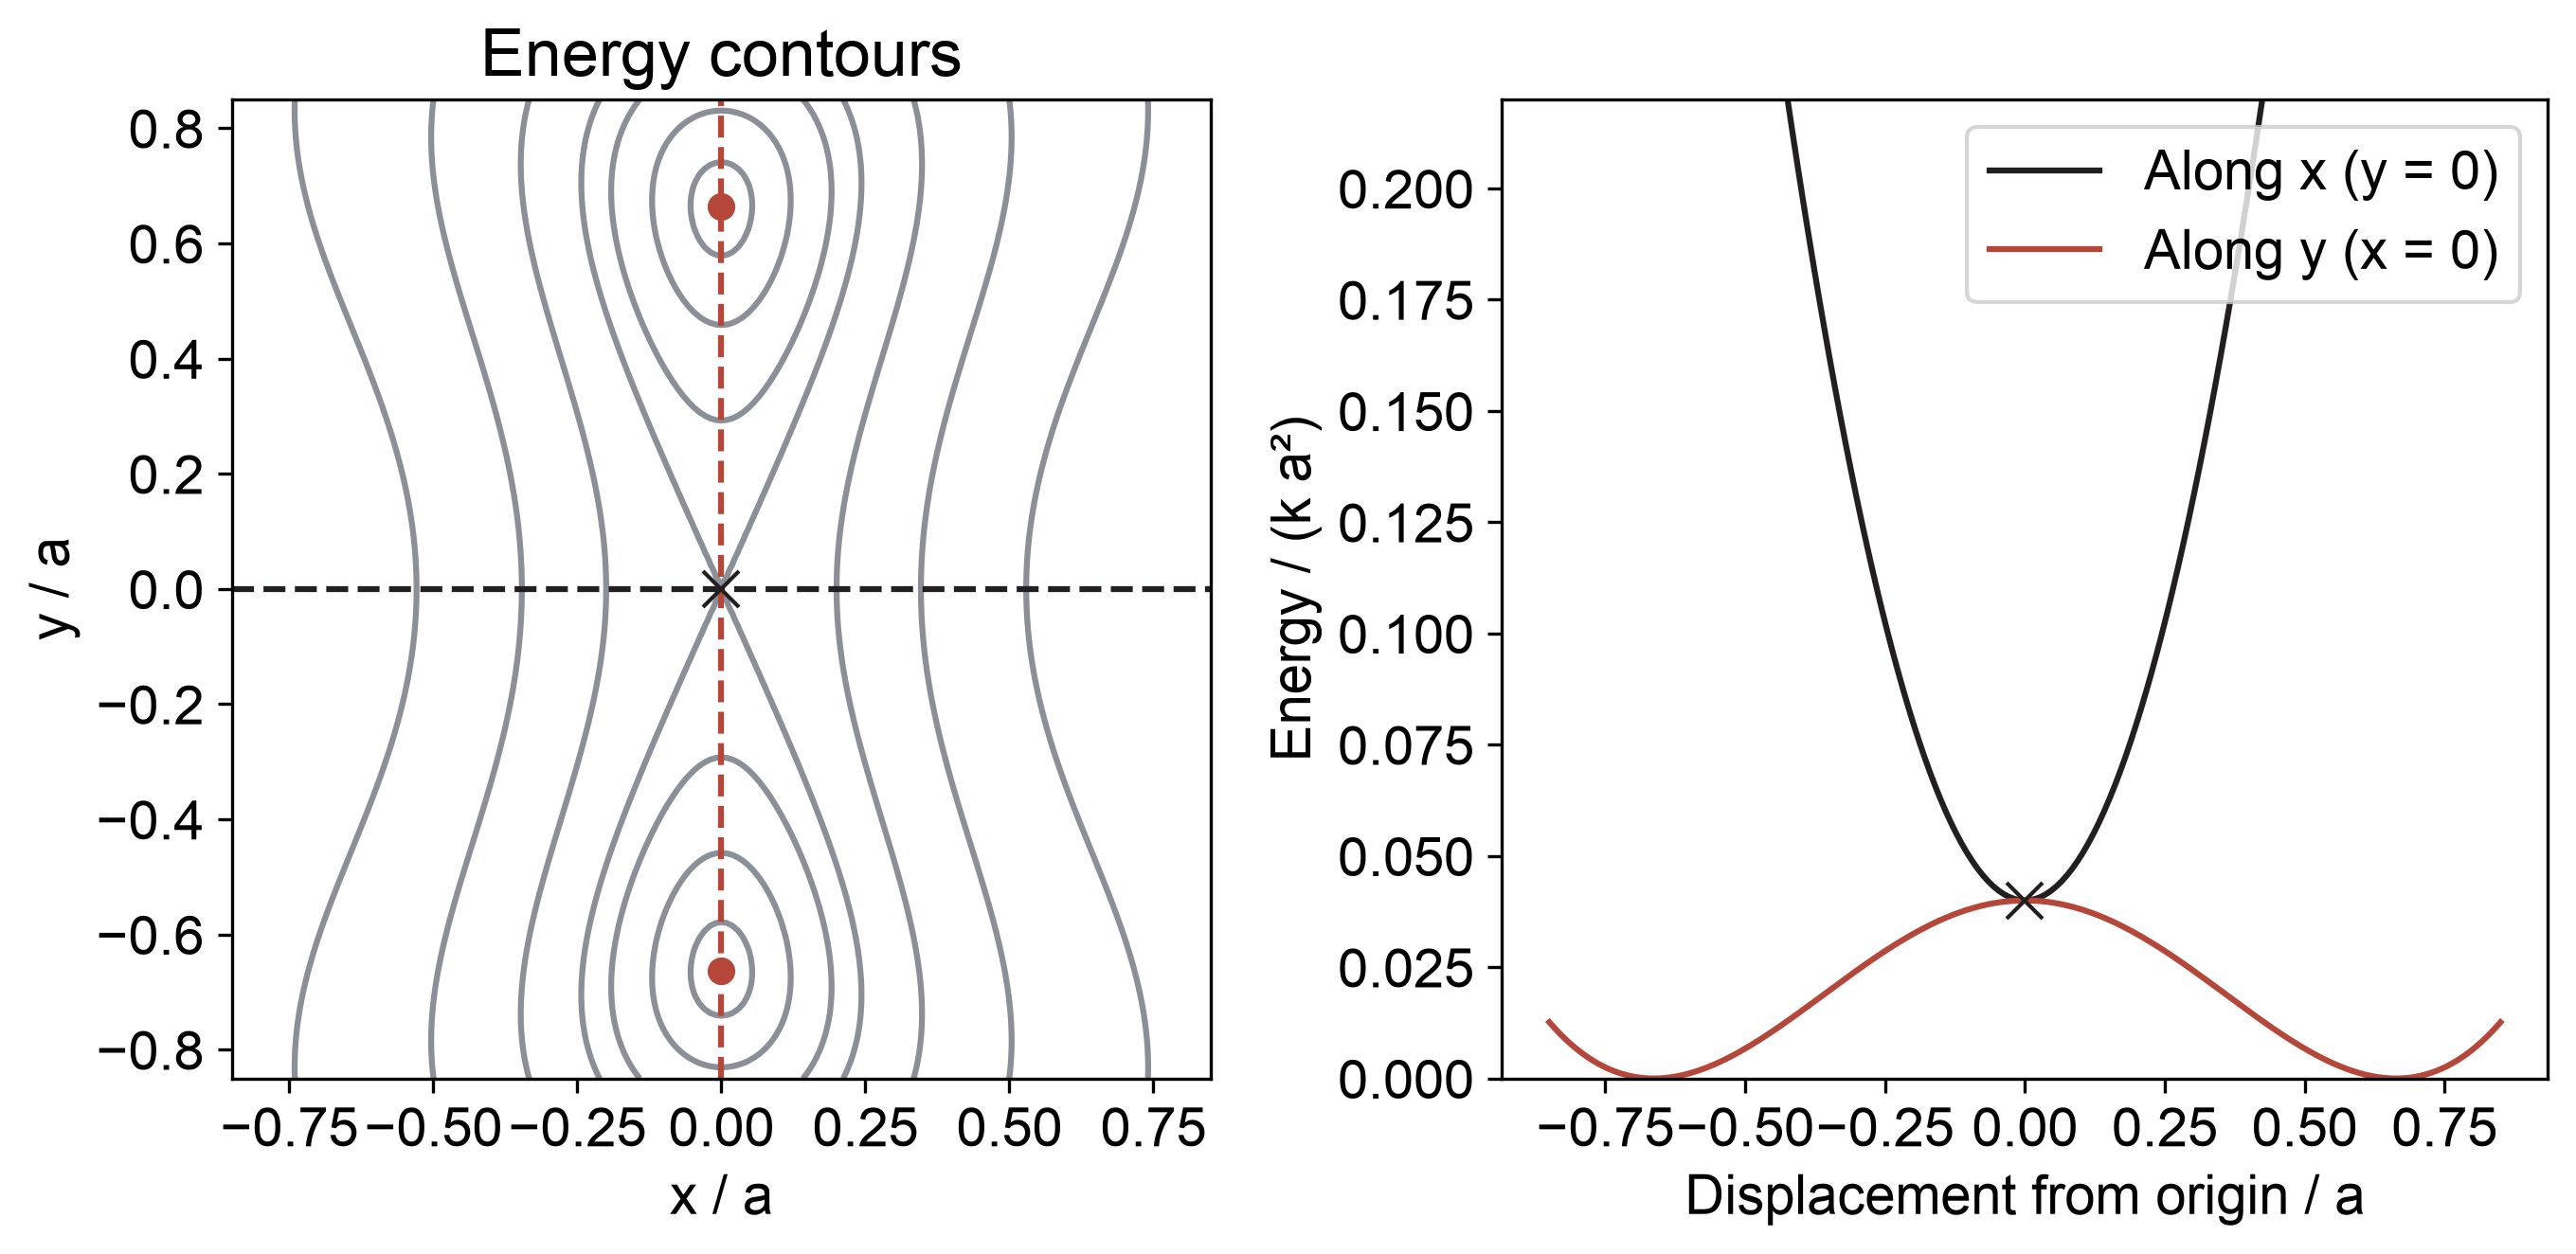
\includegraphics[width=1\linewidth,height=\textheight,keepaspectratio,alt={An energy contour map with minima above and below the origin, beside energy profiles along the horizontal and vertical axes showing opposite curvatures at the origin.}]{../../../assets/L15-energy-sections.png}

}

\caption{\label{fig-energy-sections}Energy contours of the middle atom,
with one-dimensional cuts through the central stationary point. The
horizontal cut has a minimum at the origin, while the vertical cut has a
maximum there and minima above and below it.}

\end{figure}%

\subsubsection{Applying the Newton loop}\label{applying-the-newton-loop}

Begin at \(\mathbf p_0=(0.3,0.1)\). Evaluate the gradient, solve with
the current Hessian, and update the position. The editable notebook
implements this loop:

\begin{Shaded}
\begin{Highlighting}[]
\NormalTok{p }\OperatorTok{=}\NormalTok{ np.array([}\FloatTok{0.3}\NormalTok{, }\FloatTok{0.1}\NormalTok{])}
\ControlFlowTok{for}\NormalTok{ iteration }\KeywordTok{in} \BuiltInTok{range}\NormalTok{(}\DecValTok{50}\NormalTok{):}
\NormalTok{    g }\OperatorTok{=}\NormalTok{ gradient(p, l0)}
    \ControlFlowTok{if}\NormalTok{ np.linalg.norm(g) }\OperatorTok{\textless{}} \FloatTok{1e{-}10}\NormalTok{:}
        \ControlFlowTok{break}
\NormalTok{    delta\_p }\OperatorTok{=}\NormalTok{ np.linalg.solve(hessian(p, l0), }\OperatorTok{{-}}\NormalTok{g)}
\NormalTok{    p }\OperatorTok{=}\NormalTok{ p }\OperatorTok{+}\NormalTok{ delta\_p}
\end{Highlighting}
\end{Shaded}

The call to \texttt{hessian} belongs \emph{inside} the loop because its
entries depend on the position. Keeping the initial Hessian would define
a different iteration. In either case, check the final gradient and
whether the loop reached its iteration limit before accepting the
answer.

For this starting point, Newton approaches \((0,0)\) in four
corrections. The forces cancel there, but its energy is
\(k(a-l_0)^2=0.04\) in units with \(a=k=1\). We already found
configurations with zero energy. Why has Newton stopped between them?

\subsection{Minimization with SciPy}\label{minimization-with-scipy}

\textless many of this part should be moved above\ldots\textgreater{}

The force-balance Newton loop searches for a zero gradient. An
optimization method also uses energy values to decide which trial steps
to accept. For example, a line search can shorten a proposed step until
it gives a sufficient energy decrease. This provides a way to direct the
search toward a nearby minimum.

In L07, \texttt{minimize\_scalar} took one scalar variable. Here the
energy still returns one number, but its input is an array of
coordinates, so we use
\href{https://docs.scipy.org/doc/scipy/reference/generated/scipy.optimize.minimize.html}{\texttt{scipy.optimize.minimize}}:

\begin{Shaded}
\begin{Highlighting}[]
\ImportTok{from}\NormalTok{ scipy.optimize }\ImportTok{import}\NormalTok{ minimize}

\NormalTok{result }\OperatorTok{=}\NormalTok{ minimize(energy, [}\FloatTok{0.3}\NormalTok{, }\FloatTok{0.1}\NormalTok{], args}\OperatorTok{=}\NormalTok{(l0,),}
\NormalTok{                  jac}\OperatorTok{=}\NormalTok{gradient, method}\OperatorTok{=}\StringTok{"BFGS"}\NormalTok{)}
\NormalTok{result.x       }\CommentTok{\# final coordinates}
\NormalTok{result.fun     }\CommentTok{\# energy at those coordinates}
\NormalTok{result.success }\CommentTok{\# whether this method\textquotesingle{}s stopping criterion was met}
\NormalTok{result.message }\CommentTok{\# explanation of termination}
\end{Highlighting}
\end{Shaded}

The keyword \texttt{jac} supplies the first derivative of the objective.
Since the objective is a scalar energy, that derivative is the gradient
vector. The Hessian would be supplied separately as \texttt{hess} for
methods that use it. BFGS does not require an explicit Hessian.

\subsubsection{What information do the methods
need?}\label{what-information-do-the-methods-need}

{\def\LTcaptype{none} % do not increment counter
\begin{longtable}[]{@{}
  >{\raggedright\arraybackslash}p{(\linewidth - 4\tabcolsep) * \real{0.3333}}
  >{\raggedright\arraybackslash}p{(\linewidth - 4\tabcolsep) * \real{0.3333}}
  >{\raggedright\arraybackslash}p{(\linewidth - 4\tabcolsep) * \real{0.3333}}@{}}
\toprule\noalign{}
\begin{minipage}[b]{\linewidth}\raggedright
Method
\end{minipage} & \begin{minipage}[b]{\linewidth}\raggedright
How it chooses a step
\end{minipage} & \begin{minipage}[b]{\linewidth}\raggedright
Information supplied
\end{minipage} \\
\midrule\noalign{}
\endhead
\bottomrule\noalign{}
\endlastfoot
Nelder--Mead & Compares energies at a triangle of points in 2D,
reflecting, expanding, or shrinking it & Energy only \\
Gradient descent & Moves along \(-\nabla E\), with a selected step
length & Gradient \\
Newton stationary-point iteration & Solves
\(\mathbf H\Delta\mathbf x=-\nabla E\) & Gradient and Hessian \\
BFGS & Builds a curvature approximation from successive gradients and
uses a line search & Energy and gradient \\
L-BFGS-B & Uses a limited history of gradients and can impose coordinate
bounds & Energy and gradient \\
Nonlinear conjugate gradient (CG) & Combines the current downhill
direction with information from the previous direction & Energy and
gradient \\
\end{longtable}
}

Nelder--Mead provides a derivative-free choice (Nelder and Mead 1965).
BFGS needs gradient information but can estimate it by finite
differences when we omit \texttt{jac}. That avoids supplying a
derivative function, at the cost of additional energy evaluations. For
many atomic coordinates, calculators that provide forces efficiently
make gradient-based methods especially useful.

Gradient descent and the plain Newton iteration in the table are
handwritten comparisons in our notebook. SciPy's \texttt{minimize}
offers named Newton-related methods with their own line-search or
trust-region procedures, rather than a method named simply
\texttt{Newton}.

\subsubsection{Six paths on the same
landscape}\label{six-paths-on-the-same-landscape}

No need here

\begin{figure}

\centering{

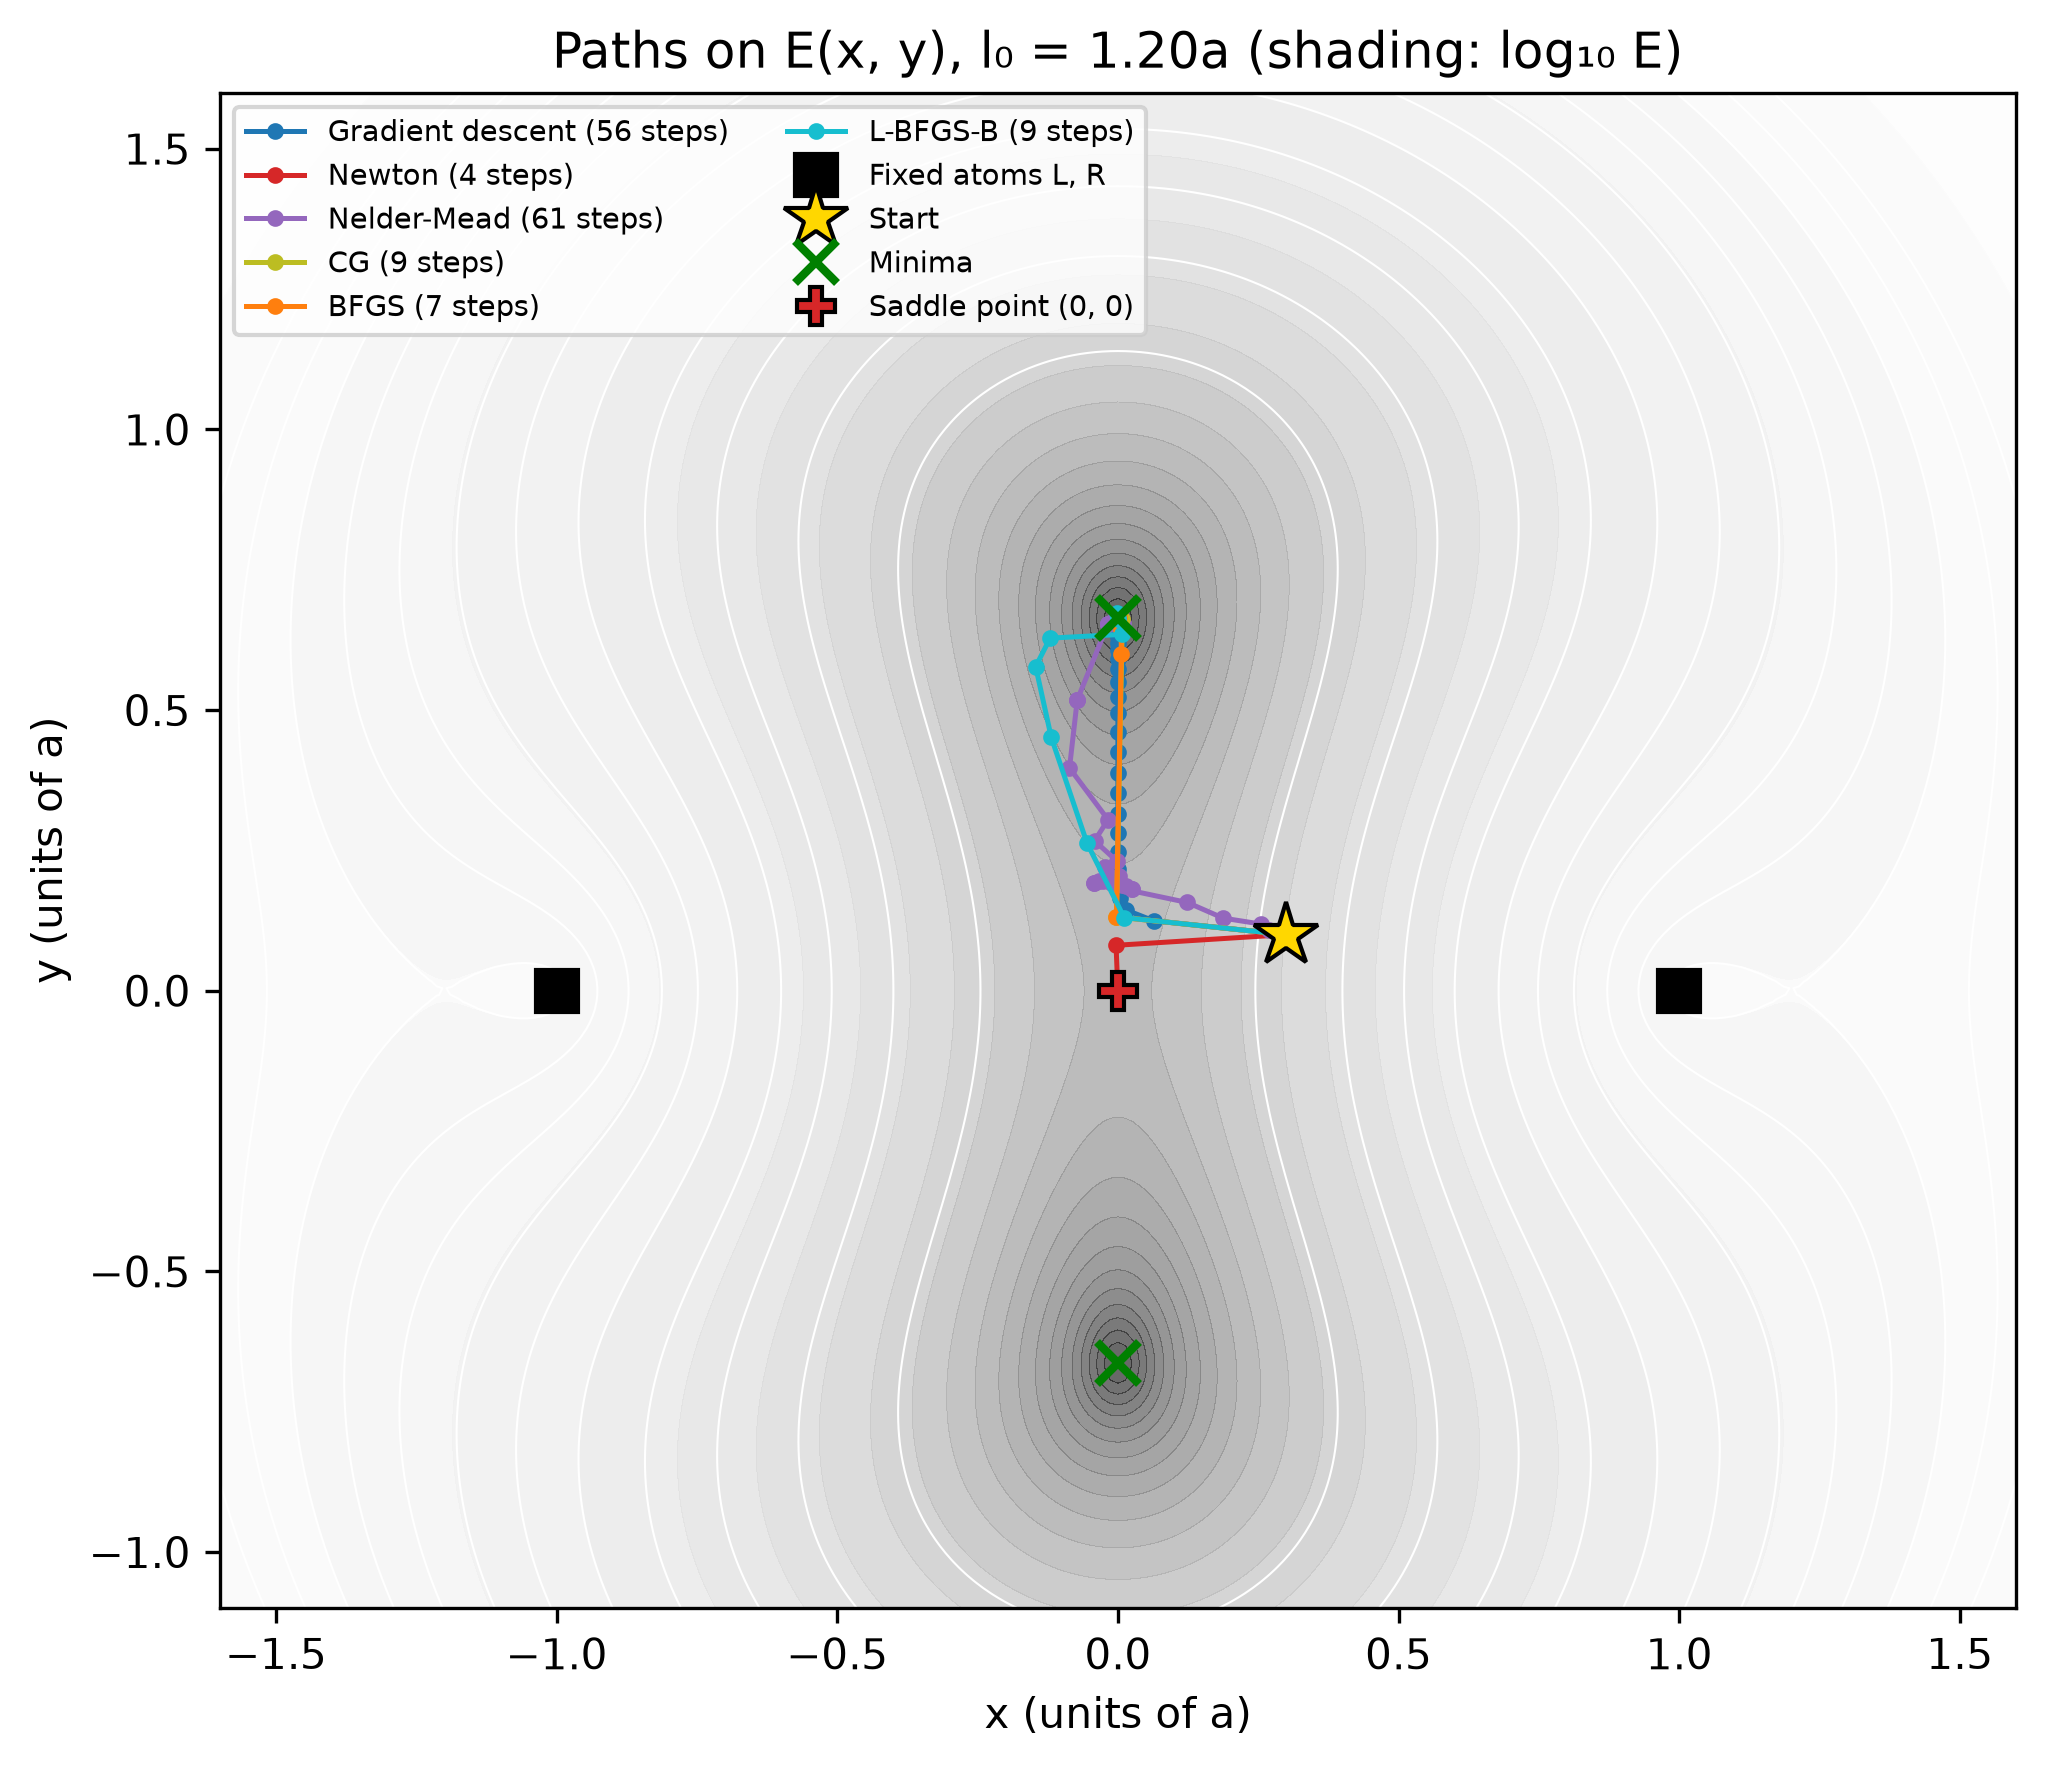
\includegraphics[width=0.95\linewidth,height=\textheight,keepaspectratio,alt={Contours of the two-minimum energy landscape with paths for gradient descent, Newton, Nelder-Mead, CG, BFGS and L-BFGS-B. Newton ends at the origin and the other paths end above it.}]{../../../assets/L15-minimizer-paths.png}

}

\caption{\label{fig-minimizer-paths}Six algorithms started at the same
position on the spring energy landscape. Newton reaches the central
stationary point, while the other five methods reach the upper minimum
for this starting point.}

\end{figure}%

The paths in Figure~\ref{fig-minimizer-paths} show that the method
changes both the route and the endpoint. From \((0.3,0.1)\), BFGS
reaches approximately \((0,0.6633)\), whereas Newton ends at the origin.
Gradient descent takes many smaller steps. A step length small enough to
remain controlled across a steep direction can give slow progress along
a shallow valley.

The notebook supplies the energy, gradient, and Hessian of the middle
atom. Handwritten gradient descent and Newton loops are compared with
SciPy's Nelder--Mead, CG, BFGS, and L-BFGS-B. With \(l_0=1.2a\) and
initial position \((0.3a,0.1a)\), Newton reaches the origin in four
corrections, while the other methods reach the upper minimum near
\((0,0.6633a)\). Changing the starting point reveals the dependence of
the final structure on the search path.

\textbf{In class:} start above the horizontal axis, then below it.
Predict which minimum a downhill method will reach. Finally, start
exactly at the origin. Does a method supplied with a zero gradient have
a direction in which to begin?

\subsubsection{How BFGS approximates
curvature}\label{how-bfgs-approximates-curvature}

Newton constructs a full Hessian at every position. BFGS instead uses
the gradients already calculated along its path. If the last
displacement was \(\mathbf s=\mathbf x^{(m+1)}-\mathbf x^{(m)}\) and the
gradient changed by \(\mathbf y=\mathbf g^{(m+1)}-\mathbf g^{(m)}\), an
approximate Hessian \(\mathbf B\) is updated to satisfy

\[
\mathbf B\mathbf s=\mathbf y.
\]

This is the multidimensional counterpart of estimating a derivative from
a secant slope. The displacement and gradient change give curvature
information along the direction actually travelled. With suitable
curvature and line-search conditions, BFGS maintains an approximation
that gives downhill search directions. For this example it avoids the
saddle reached by the unrestricted Newton step.

A dense Hessian for 1000 freely moving atoms has \(3000\times3000\)
entries. Constructing and solving with that matrix repeatedly can
dominate the calculation. \textbf{Limited-memory BFGS} stores a short
history of displacements and gradient changes instead of the full
matrix. These methods let us extend the same optimization idea to far
more coordinates without explicitly building every second derivative.

\subsection{The stationary point between the
minima}\label{the-stationary-point-between-the-minima}

At the origin, the two compressed springs push equally in opposite
directions, so the gradient is exactly zero. Move the atom slightly in
\(x\): one spring becomes more compressed and the other less compressed.
Their net force pushes it back, and the energy rises. Move it slightly
in \(y\): both springs lengthen toward their natural length, lowering
the energy and pushing the atom farther from the origin.

The origin is a \textbf{saddle point}. A saddle has directions in which
the energy rises and directions in which it falls. The two cuts in
Figure~\ref{fig-energy-sections} make that distinction visible even
though both first derivatives vanish at their intersection. Newton met
its root-finding goal there, but the atom can still reduce its energy by
moving vertically.

A minimizer can also stop at a saddle, particularly when an exactly
symmetric starting configuration gives no downhill gradient. Its success
flag records an algorithmic stopping criterion. Depending on the method,
this can involve gradient size, step size, or changes in energy. We must
interpret that criterion before drawing a conclusion about structural
stability.

\subsection{From the middle atom to an atomic
cluster}\label{from-the-middle-atom-to-an-atomic-cluster}

A cluster has more coordinates, but a minimizer still needs the same
basic information: an energy, its gradient, and a starting structure.
Atomistic packages arrange these through a structure object, an
energy-and-force calculator, and an optimizer. The calculator may
evaluate a pair potential or a much more detailed electronic-structure
model.

The \href{https://ase-lib.org/}{Atomic Simulation Environment} provides
these objects. The editable example below starts with 13 argon atoms
near an icosahedron, displaces them, and relaxes the cluster with BFGS,
LBFGS, and FIRE. \textbf{FIRE}, the fast inertial relaxation engine,
moves atoms using forces and an adaptive, damped dynamical update. This
is an extension of the two-coordinate exercise: the optimizer now moves
39 coordinates, while the LJ calculator supplies energies and forces.
ASE's \texttt{fmax} criterion uses the largest \textbf{force-vector norm
on an atom}, in eV/Å.

\begin{figure}

\centering{

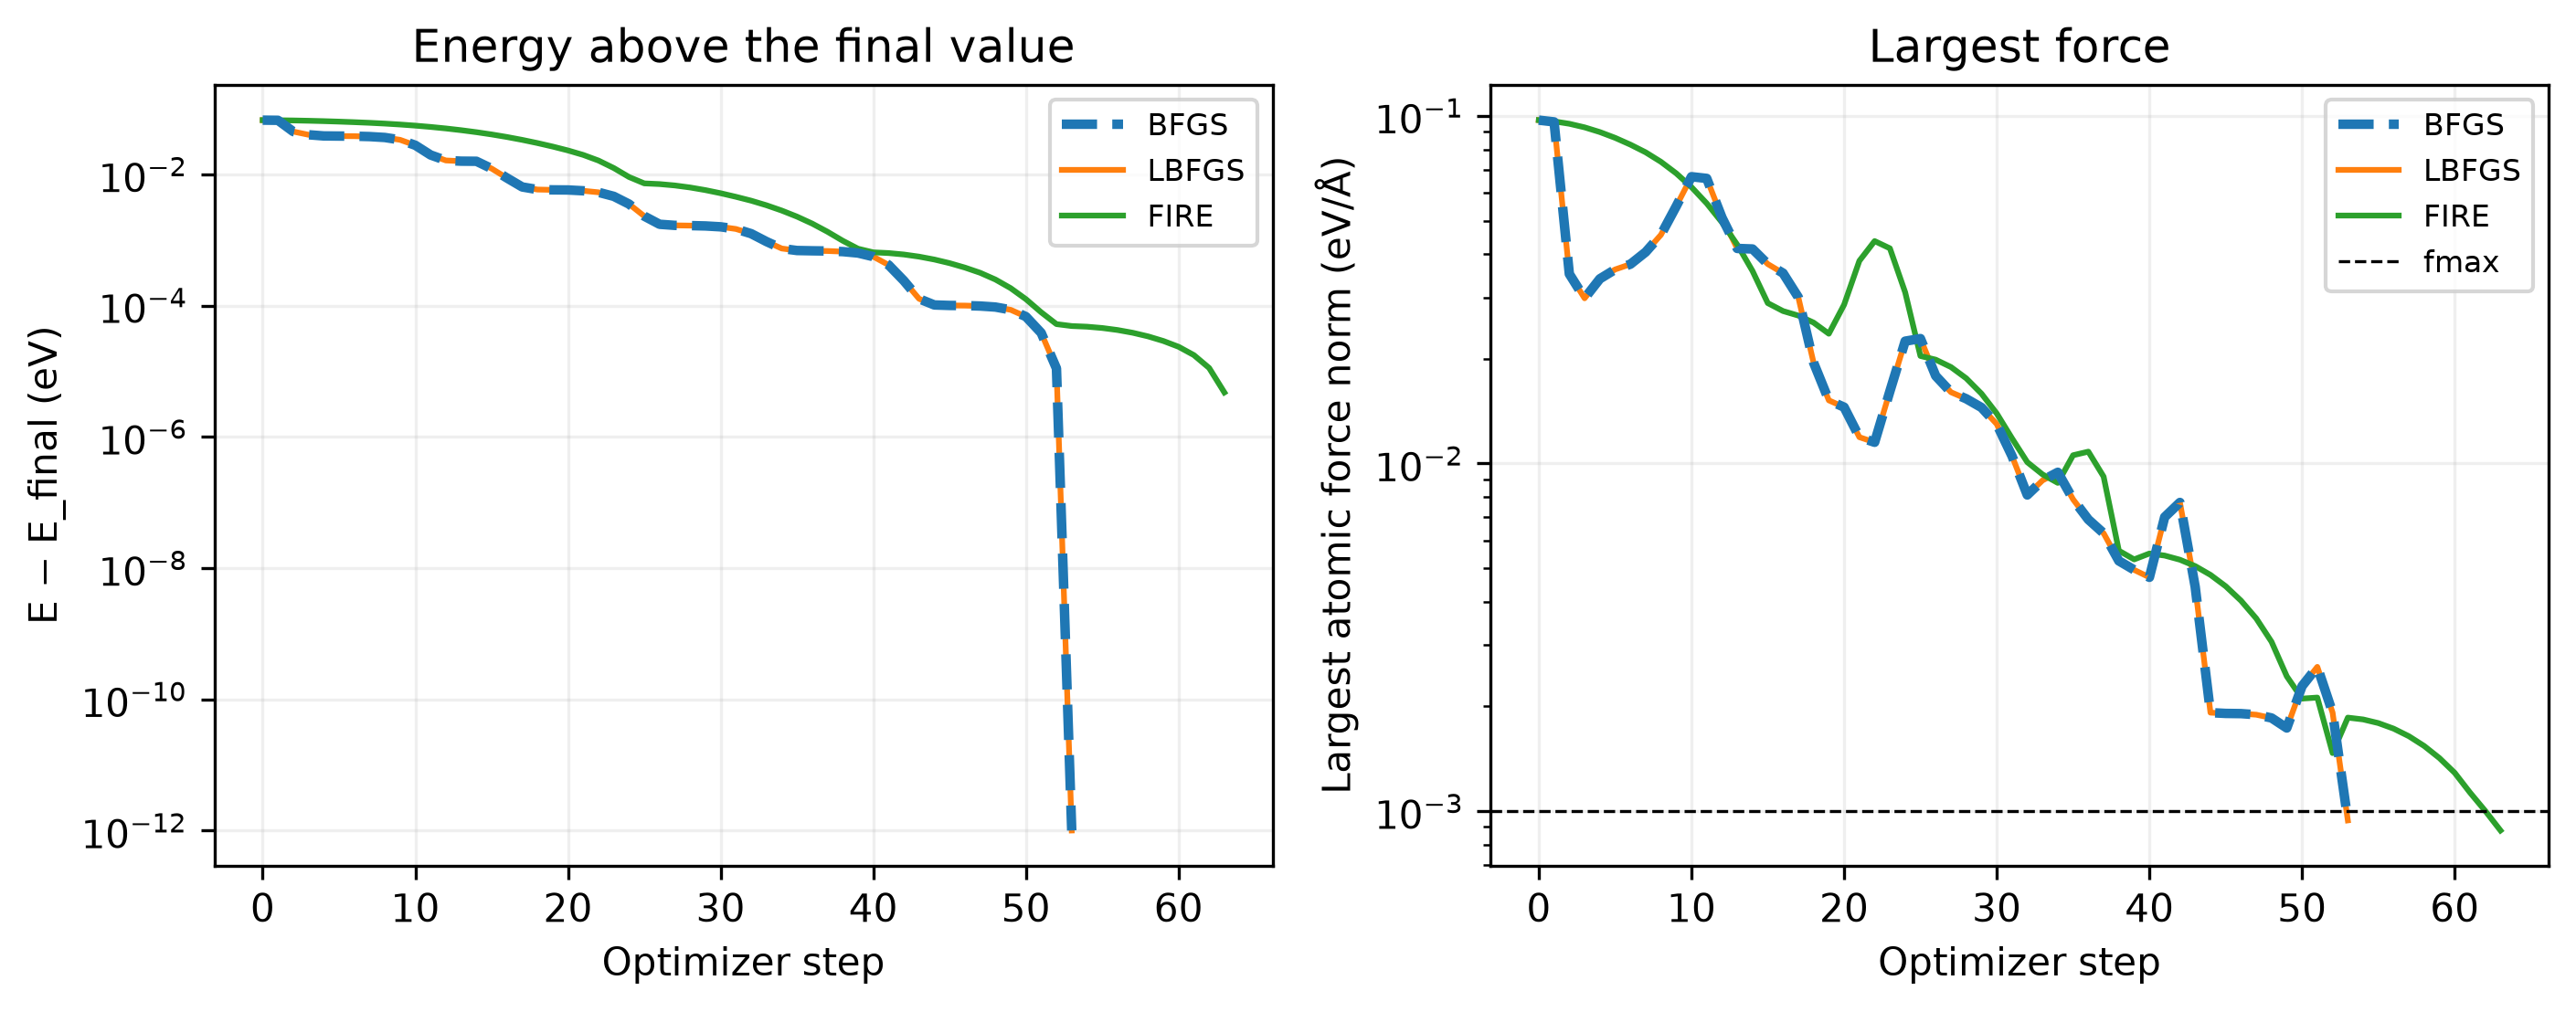
\includegraphics[width=1\linewidth,height=\textheight,keepaspectratio,alt={Two convergence plots for ASE BFGS, LBFGS and FIRE, showing energy above the final value and the recorded force measure against optimization step.}]{../../../assets/L15-ase-relaxation.png}

}

\caption{\label{fig-ase-relaxation}Relaxation of a displaced 13-atom
argon cluster. The energy and force measures decrease as three ASE
optimizers return the atoms to a nearby minimum.}

\end{figure}%

The notebook combines an atomic structure, an LJ calculator for argon or
an EMT calculator for copper, and ASE optimizers. In the supplied
13-atom argon case, all three methods reach approximately \(-0.4566\)
eV. The optimizer stops when the maximum norm of an atomic force is
below \(10^{-3}\) eV/Å. The same division between physical model and
numerical optimizer applies to larger structures.

The central difficulty now becomes harder to inspect by eye. For the
middle atom, two plotted energy cuts revealed the saddle. A cluster can
move along combinations of many coordinates, so we need a matrix-based
way to find any downhill displacement that remains after relaxation.

\subsection{What to keep}\label{what-to-keep}

\begin{enumerate}
\def\labelenumi{\arabic{enumi}.}
\tightlist
\item
  The gradient is \(\nabla E\), the force is \(-\nabla E\), and the
  force Jacobian is \(-\mathbf H\).
\item
  Newton's stationary-point equation is
  \(\mathbf H\Delta\mathbf x=-\nabla E\). It reaches the minimum in one
  step for the supported harmonic chain's quadratic energy.
\item
  Harmonic springs can still give a position-dependent Hessian when
  their lengths depend nonlinearly on Cartesian coordinates.
\item
  \texttt{minimize} accepts a vector of coordinates and a scalar energy.
  Methods differ in whether they use energies, gradients, or Hessians.
\item
  Zero force establishes a stationary point. Energy changes around that
  point distinguish a minimum from a saddle.
\end{enumerate}

\subsection{Check your understanding}\label{check-your-understanding}

\begin{enumerate}
\def\labelenumi{\arabic{enumi}.}
\tightlist
\item
  Why is the Jacobian of the net force the negative of the Hessian of
  the energy?
\item
  Explain why the two-dimensional spring system needs an updated Hessian
  even though both spring constants remain fixed.
\item
  Find the two zero-energy configurations for \(l_0=1.3a\) without
  running an optimizer.
\item
  A calculator supplies only energies. Which method in the table can use
  them directly, and how could BFGS obtain the gradient information it
  needs?
\item
  Why can Newton converge to the origin of the compressed spring system?
  What additional observation shows that this point is unstable?
\end{enumerate}

\subsection{Next}\label{next}

For one atom moving in a plane, we can draw the energy and find a
downhill direction. L16 asks how to make that test using the Hessian,
including when the stable and unstable directions no longer line up with
the coordinate axes. The resulting eigenvalue problem provides a
stability test for high-dimensional structures.

\protect\phantomsection\label{refs}
\begin{CSLReferences}{1}{1}
\bibitem[\citeproctext]{ref-nelder1965simplex}
Nelder, John A., and Roger Mead. 1965. {``A Simplex Method for Function
Minimization.''} \emph{The Computer Journal} 7 (4): 308--13.
\url{https://doi.org/10.1093/comjnl/7.4.308}.

\end{CSLReferences}




\end{document}
